\clearpage
\section{Within-image SPI reset and MISO control: 14--15 November 2026}
The combined image \texttt{30096dcc} provides independent parser reset (bit 0)
and MISO clamp (bit 1) controls at IPbus 305. A positive baseline is established
before comparison. Stimulus remains divider 601/read 0. Kasli, external clock
profiles and buffer directions/OE remain unchanged; there is no FPGA
programming between conditions within a cohort.

\subsection{Primary reset-only reversal}
Mode 0$\rightarrow$1$\rightarrow$0 changes only reset bit 0; the explicit MISO
clamp remains disabled. The original parser reset branch retains shift data
with MSB 0, so raw MISO becomes constant zero naturally. Direct state probes
verify that the parser is actually held while SCK still clocks its input.
\begin{center}\begin{tabular}{lrr}\toprule
Stage & Mode & SYS resets / frames\\\midrule
Selected normal baseline &0&2/2\\
R1: reset only &1&0/6\\
A1: release reset &0&6/6\\
C: active parser, MISO clamp0 &2&0/6\\
A2: remove clamp &0&6/6\\
R2: reset only &1&0/6\\
A3: release reset &0&6/6\\\bottomrule\end{tabular}\end{center}
Initial search across reads 0/1/2 gave 6/6 reset witnesses; read 0 was selected
after two witnesses. There are 44 complete windows: 42 SPI frames and 2 idle controls.
All replies match the expected diagnostic value(zero while held or clamped).
All sampled control flags are verified. Parser count reaches 31 in normal and
clamp-only frames, and stays 0 with reading 0 during reset-only frames.

\subsection{Independent MISO control}
A separate cohort of the identical bitstream ran mode 2 (clamp-only) and
mode 3 (reset+clamp), interleaved C1--B1--C2--B2--C3--A-return. Each block has
six frames: active/clamped C total 0/18 resets, held/clamped B total 0/12,
normal A-return 6/6. Its selected read 0 baseline was 2/2 (mixed search 5/6).
This cohort also contains 44 windows/42 frames/2 idle. A configuration occurred
between cohorts; neither comparison mixes conditions across that boundary.

\textbf{Reset-only suppressed the observed fault, and reset release reproduced
it. Reset is not necessary for suppression: MISO clamp alone works while the
parser remains active.} A unique parser-state-machine cause is not established.
The experiment identifies MISO-dependent behavior, not a proven short, driver,
contention or reference-clock fault. It also does not distinguish constant
levels from switching. Internal MISO data and received payloads are recorded,
not a continuous electrical pad waveform.

\subsection{Provenance and final state}
The observer uses nominal 40.0787 MHz MCLK1 independent of SYS reset. First 8 ARM
ticks are settling; sampled multibit fields are not atomic, and a common
watch/reference stop is invisible. Frozen raw records, not network timeouts,
qualify resets. Read-only recovery is bounded; writes are not blindly replayed.
Candidate WNS 0.019 ns/WHS 0.061 ns, no DRC errors/critical warnings. Simulations
cover active/clamped/held separation, reset-only release and observer readout.

One initial attempt failed in Python result construction before any SPI frame
and restored the original image. The first completed cohort launcher reported 143
after complete saved results/restoration; subsequent fresh checks are healthy.
Primary reset-only acquisition exited 0. All logs and execution receipts are
retained. Both cohorts restore exact \texttt{c7531465}; final tailcheck verifies
power, frontend 0xfff and driven Kasli SPI. Physical ADC bankA on all 12 channels
passed first postflight attempts. No explicit external PLL, MCU, CPLD, flash
or analog programming. The known intermittent HDMI/SYS fault remains open;
normal responses are restored, not replaced by permanent zero data.
Evidence:\texttt{system/evidence-spi-ab-20261115}.
\clearpage
\begin{figure}[p]\centering
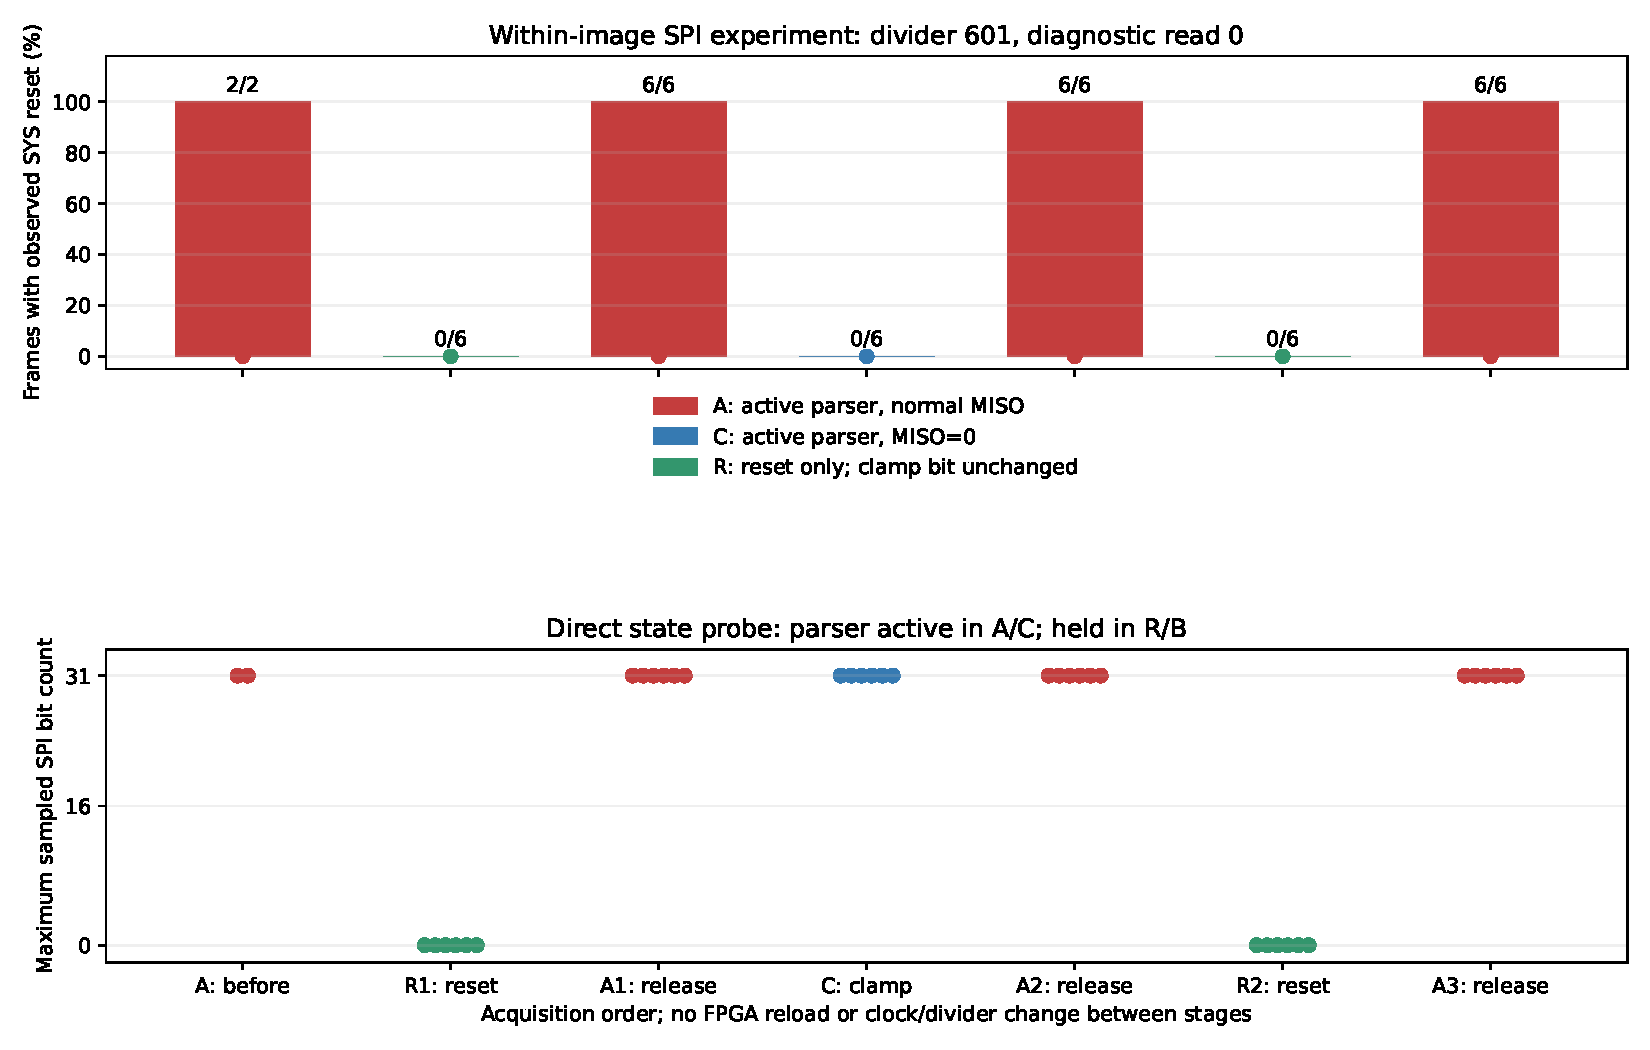
\includegraphics[width=\textwidth,height=.85\textheight,keepaspectratio]{spi-ab-reset-only.pdf}
\caption{Primary cohort. Only reset bit changes between A and R. Clamp-only C
is an independent control; no programming or clock change within this sequence.}
\end{figure}\clearpage
\begin{figure}[p]\centering
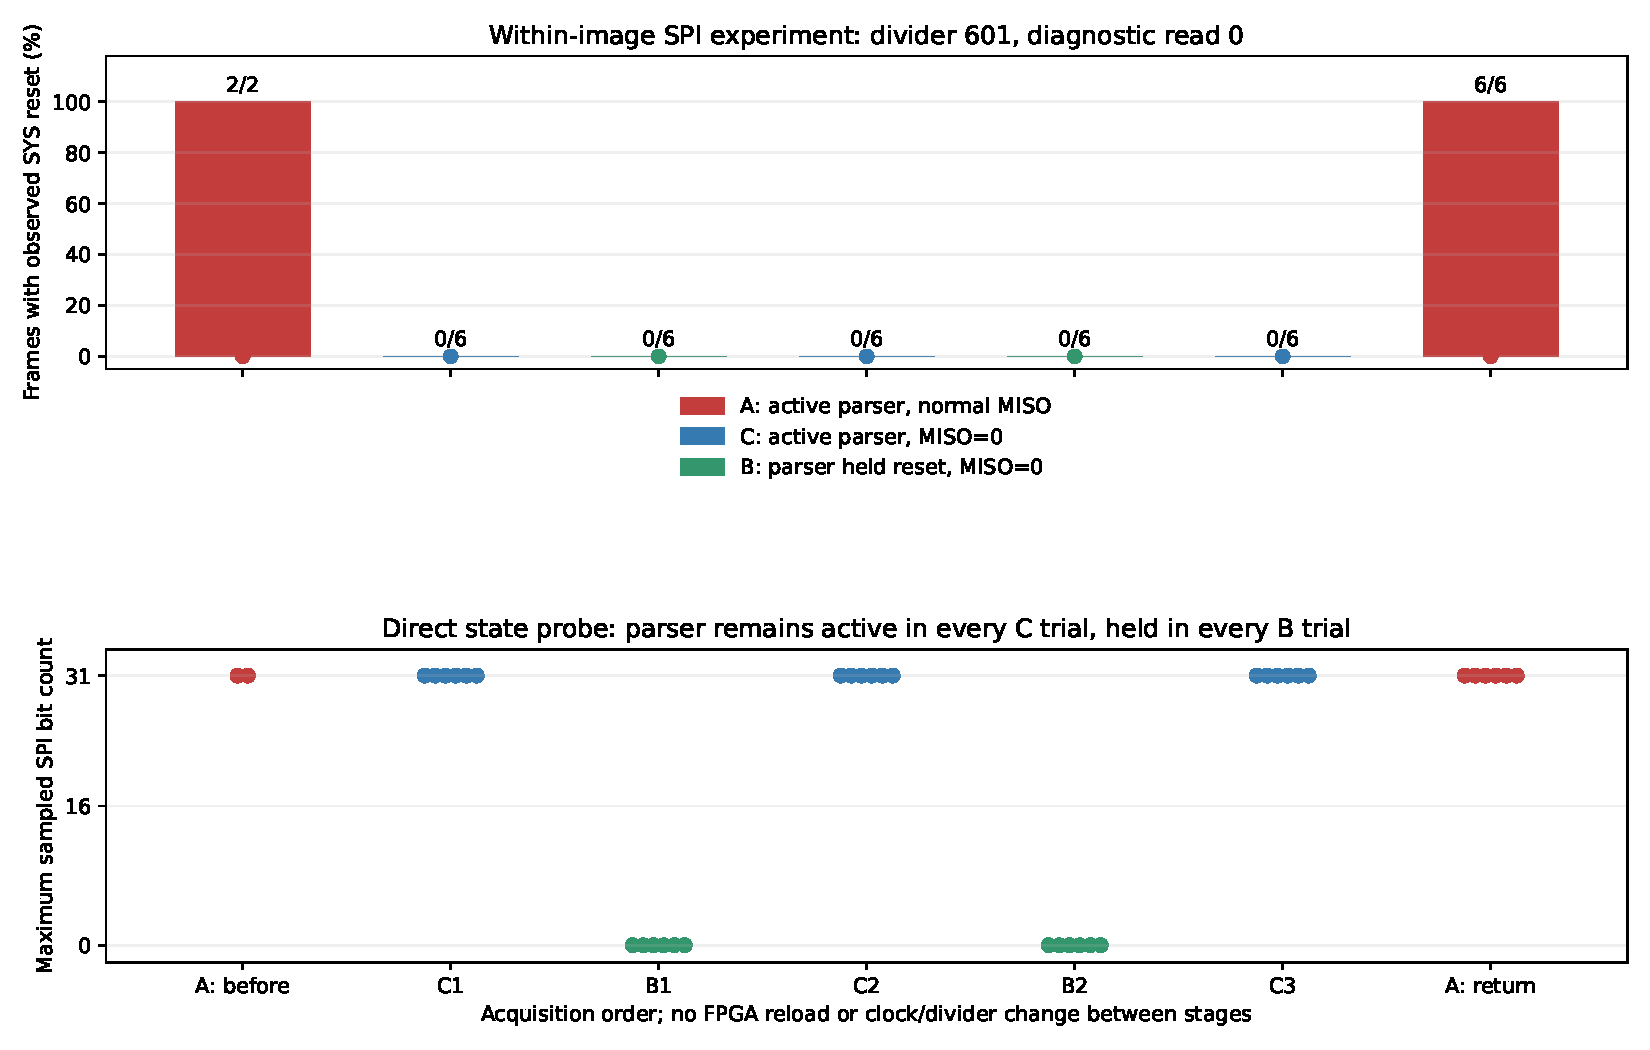
\includegraphics[width=\textwidth,height=.85\textheight,keepaspectratio]{spi-ab-clamp.pdf}
\caption{Separate matched-clamp cohort. Active parser with zero MISO suppresses
observed resets without holding the parser. No programming between these stages.}
\end{figure}\clearpage
